\documentclass[conference]{IEEEtran}
\IEEEoverridecommandlockouts

\usepackage{cite}
\usepackage{amsmath,amssymb,amsfonts}
\usepackage{algorithmic}
\usepackage{graphicx}
\usepackage{textcomp}
\usepackage{xcolor}
\usepackage{url}
\usepackage{fancyhdr}

\fancypagestyle{paperfooter}{
    \fancyhf{}
    \fancyfoot[C]{\footnotesize Makalah IF2211 Strategi Algoritma, Semester II Tahun 2025/2026}
    \renewcommand{\headrulewidth}{0pt}
    \renewcommand{\footrulewidth}{0pt}
}
\pagestyle{paperfooter}

\def\BibTeX{{\rm B\kern-.05em{\sc i\kern-.025em b}\kern-.08em
    T\kern-.1667em\lower.7ex\hbox{E}\kern-.125emX}}

\begin{document}

\title{Efficient Transformer Compression via Dynamic Programming-Based Mixed-Precision Bit-Width Allocation}

\author{
\IEEEauthorblockN{Athilla Zaidan Zidna Fann -- 13524068}
\IEEEauthorblockA{
\textit{Program Studi Teknik Informatika}\\
\textit{Sekolah Teknik Elektro dan Informatika}\\
Institut Teknologi Bandung, Jl. Ganesha 10 Bandung 40132, Indonesia\\
athillazaidanstudy@gmail.com, 13524068@std.stei.itb.ac.id}
}

\maketitle
\thispagestyle{paperfooter}

\begin{abstract}
Transformer models deliver strong performance in natural language processing, but their memory footprint makes deployment difficult on resource-constrained devices. This paper studies mixed-precision quantization as an optimization problem: each Transformer layer is assigned a bit-width under a model-size budget while minimizing estimated accuracy degradation. The proposed method formulates bit-width allocation as a multiple-choice knapsack problem and solves it using Dynamic Programming. Experiments on BERT-base with fake quantization show that the proposed allocator selects configuration $[4,4,8,8,4,8,8,8,8,4,4,4]$ under budget 72, achieving an estimated 5.33$\times$ compression ratio with 0.044 accuracy loss from an 89.4\% baseline.
\end{abstract}

\begin{IEEEkeywords}
Dynamic Programming, Transformer Compression, Mixed-Precision Quantization, Bit-Width Allocation, Model Compression
\end{IEEEkeywords}

\section{Introduction}
Transformer-based language models have become the dominant architecture for modern natural language processing because they can capture long-range dependencies and transfer knowledge effectively across downstream tasks. BERT and its variants are widely used for classification, question answering, and semantic representation tasks. However, this accuracy comes with a substantial computational cost. BERT-base contains twelve Transformer encoder layers and millions of parameters, and the default floating-point representation typically uses 32 bits per weight. When such models are deployed on mobile devices, embedded systems, or low-cost servers, memory consumption and inference cost become practical bottlenecks rather than secondary implementation details.

Model compression addresses this limitation by reducing the storage and computation required during inference. Quantization is one of the most direct compression techniques: model weights that are originally represented as 32-bit floating-point numbers are mapped into lower-precision representations such as 8-bit, 4-bit, or 2-bit values. This approach can significantly reduce model size because the number of bits used to store each parameter decreases. For example, replacing 32-bit weights with 8-bit weights theoretically reduces the weight storage requirement by a factor of four. For Transformer models with repeated layers and large feed-forward blocks, this reduction is especially attractive.

Uniform quantization applies the same bit-width to every layer. Although simple, this strategy ignores the fact that not all layers have the same sensitivity to precision reduction. Some Transformer layers can tolerate aggressive quantization with only small accuracy degradation, while other layers may suffer large performance drops when forced into very low precision. This observation motivates mixed-precision quantization, in which each layer is allowed to use a different bit-width. Sensitive layers can remain at higher precision, while less sensitive layers can be compressed more aggressively. The challenge is no longer merely how to quantize a layer, but how to choose the best bit-width configuration across all layers.

The bit-width allocation problem has a combinatorial structure. If a model has $L$ layers and each layer can choose one bit-width from a set $Q = \{2,4,8\}$, then the search space contains $|Q|^L$ possible configurations. A twelve-layer BERT-base encoder already has $3^{12} = 531{,}441$ possible layer-wise assignments for the Transformer blocks alone. Larger Transformer models make exhaustive search increasingly unattractive. More importantly, the allocation decision must satisfy a global model-size budget: choosing a high bit-width for one layer consumes budget that could have been used by another layer. Therefore, locally optimal decisions do not always produce the best global configuration.

This paper formulates mixed-precision bit-width allocation as a constrained optimization problem. Each layer corresponds to a stage, each bit-width choice corresponds to a decision, the estimated size of the quantized layer corresponds to a cost, and the measured accuracy degradation caused by fake quantization corresponds to a loss. The objective is to minimize the total estimated accuracy loss while ensuring that the total model size does not exceed a predefined budget. This formulation is equivalent in structure to the multiple-choice knapsack problem, because exactly one option must be selected from each layer group.

Dynamic Programming is used to solve the allocation problem systematically. Instead of evaluating every complete configuration independently, the algorithm builds optimal partial solutions layer by layer for each possible budget value. The state $DP[i][b]$ represents the minimum estimated accuracy loss after assigning bit-widths to the first $i$ layers using at most budget $b$. By reusing subproblem solutions, the method avoids redundant computation and guarantees the best configuration under the additive loss assumption. The selected bit-width configuration is then reconstructed through backtracking from the DP table.

The experimental framing of this work uses BERT-base as the target Transformer model and fake quantization to estimate layer-wise sensitivity. In fake quantization, floating-point weights are rounded to a limited number of representable levels and then dequantized back to floating-point values for evaluation. This procedure does not provide hardware-level acceleration by itself, but it offers a controlled way to measure the effect of reduced precision on model behavior. The resulting sensitivity table becomes the input to the Dynamic Programming allocator. The proposed method is compared against uniform quantization and a greedy allocation baseline.

The main contribution of this paper is not a new quantization kernel or a new Transformer architecture. Instead, this work demonstrates that a classical algorithmic technique, Dynamic Programming, can be used to make mixed-precision quantization decisions in a clear, deterministic, and budget-aware manner. The contributions are threefold: first, the paper formulates Transformer bit-width allocation as a multiple-choice knapsack-style optimization problem; second, it applies Dynamic Programming to recover the optimal layer-wise bit configuration under a size constraint; third, it compares the resulting allocation with uniform and greedy baselines to analyze the trade-off between compression ratio and accuracy preservation.

\section{Theoretical Foundation}
\subsection{Transformer Architecture}
Transformer models were introduced as an attention-based architecture that removes recurrent computation and instead relies on self-attention to model dependencies between tokens \cite{transformer}. Given an input sequence, each token is projected into query, key, and value vectors. Attention scores are computed by comparing queries with keys, and the resulting weights are used to aggregate value vectors. The scaled dot-product attention mechanism is defined as
\begin{equation}
\mathrm{Attention}(Q,K,V)=\mathrm{softmax}\left(\frac{QK^T}{\sqrt{d_k}}\right)V,
\end{equation}
where $Q$, $K$, and $V$ denote query, key, and value matrices, and $d_k$ is the dimensionality of the key vectors. Multi-head attention repeats this operation in several representation subspaces, allowing the model to capture different linguistic relations simultaneously.

Encoder-based Transformer models such as BERT use stacked Transformer encoder blocks to produce contextual token representations \cite{bert}. Each encoder block contains multi-head self-attention, a feed-forward network, residual connections, and layer normalization. For a sequence classification task, the contextual representation of a special classification token is typically passed to a classifier head. This stacked structure is important for compression because each block contains large parameter matrices whose precision can be reduced independently.

\subsection{BERT-base as Target Model}
BERT is an encoder-only Transformer model pretrained using masked language modeling and next sentence prediction \cite{bert}. The BERT-base configuration contains twelve Transformer encoder layers, making it substantially larger than compact distilled variants while still feasible to evaluate in a notebook environment. This makes BERT-base suitable for studying mixed-precision allocation: the model is large enough for the combinatorial search space to be meaningful, yet small enough for controlled fake-quantization experiments.

In this paper, the mixed-precision allocation problem focuses on the twelve Transformer encoder layers of BERT-base. The embedding layer and classifier head are treated as fixed components so that the optimization remains centered on repeated Transformer blocks. This scope keeps the problem mathematically clear: each optimized layer must receive exactly one bit-width from a predefined set, and the complete allocation determines the compressed representation of the Transformer stack.

\begin{figure*}[htbp]
\centerline{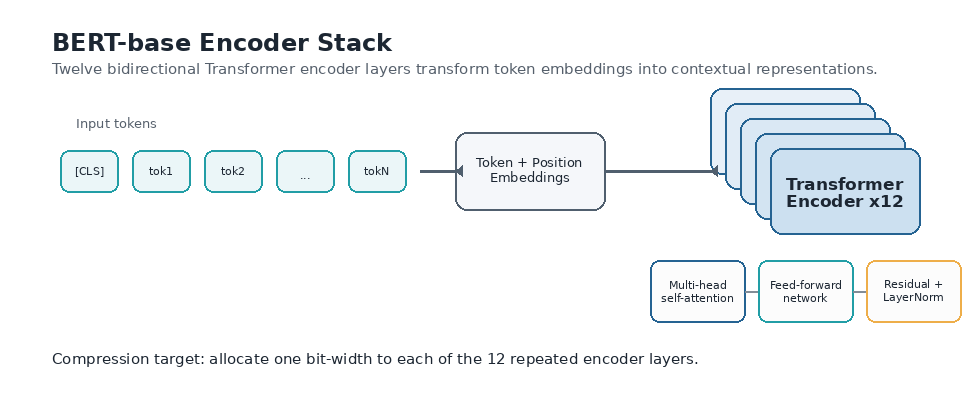
\includegraphics[width=0.86\textwidth]{figures/bert_encoder_stack.png}}
\caption{BERT-base encoder stack used as the compression target. The diagram is redrawn from the Transformer and BERT architecture concepts in \cite{transformer}, \cite{bert}.}
\label{fig:bertstack}
\end{figure*}

\subsection{Model Quantization}
Quantization reduces the numerical precision used to represent model parameters. A full-precision neural network typically stores weights as 32-bit floating-point values. Quantization maps these values to a smaller set of representable levels, such as 8-bit, 4-bit, or 2-bit integers. For a weight tensor $W$, a simple uniform affine quantization can be expressed as
\begin{equation}
W_q = \mathrm{round}\left(\frac{W}{s}\right),
\end{equation}
\begin{equation}
\hat{W} = sW_q,
\end{equation}
where $s$ is a scale factor, $W_q$ is the quantized tensor, and $\hat{W}$ is the dequantized tensor used to approximate the original weights. Lower bit-widths provide fewer representable levels, causing larger rounding errors but reducing memory cost.

For a signed symmetric quantizer with $b$ bits, the number of quantization levels is approximately
\begin{equation}
N_b = 2^b - 1.
\end{equation}
The scale can be derived from the maximum absolute weight value:
\begin{equation}
s = \frac{\max(|W|)}{2^{b-1}-1}.
\end{equation}
This formulation shows the basic trade-off. Larger $b$ produces a finer grid and lower quantization error, while smaller $b$ produces stronger compression at the risk of higher accuracy loss.

\subsection{Fake Quantization}
Fake quantization simulates low-precision weights while keeping computation in floating point. The weights are rounded to quantized levels and then dequantized before inference. Therefore, fake quantization does not directly provide hardware acceleration, but it allows the impact of reduced precision to be evaluated without implementing custom 2-bit or 4-bit kernels.

\begin{figure*}[htbp]
\centerline{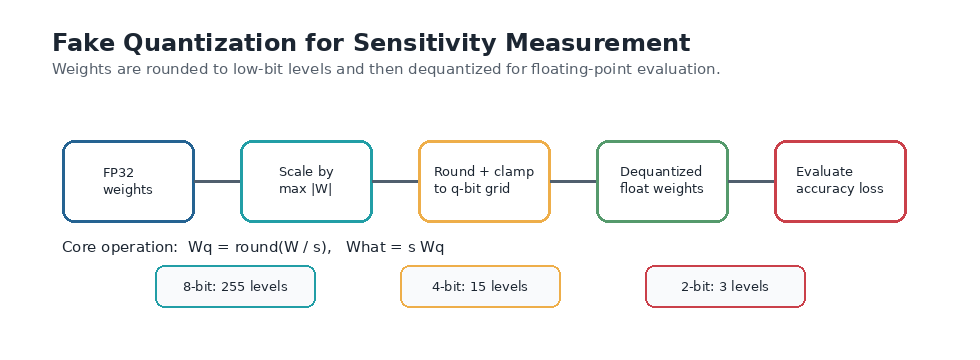
\includegraphics[width=0.84\textwidth]{figures/fake_quant_pipeline.png}}
\caption{Fake quantization pipeline used for measuring layer-wise sensitivity. The low-bit representation is simulated through rounding and dequantization, while evaluation still uses floating-point execution.}
\label{fig:fakequant}
\end{figure*}

This property is useful for layer-wise sensitivity analysis. For each Transformer layer $i$ and bit-width $q$, the layer can be fake-quantized while the rest of the model remains unchanged or follows a controlled configuration. The model is then evaluated on a validation set, and the accuracy degradation becomes a sensitivity estimate:
\begin{equation}
d_i(q) = A_{\mathrm{base}} - A_i(q),
\end{equation}
where $A_{\mathrm{base}}$ is the full-precision validation accuracy and $A_i(q)$ is the validation accuracy when layer $i$ is evaluated under bit-width $q$. A larger value of $d_i(q)$ indicates that the layer is more sensitive to that precision level.

\subsection{Mixed-Precision Quantization}
Uniform quantization assigns the same bit-width to all layers. Mixed-precision quantization generalizes this strategy by allowing each layer to choose a different bit-width. If the model has $L$ optimized layers and the available bit-width set is $Q=\{2,4,8\}$, then a mixed-precision configuration is represented as
\begin{equation}
\mathbf{q} = [q_1,q_2,\ldots,q_L], \quad q_i \in Q.
\end{equation}
For example, a twelve-layer configuration $[4,4,8,8,4,8,8,8,8,4,4,4]$ keeps several layers at 8-bit precision while compressing the remaining layers to 4-bit.

The motivation for mixed precision is that Transformer layers do not contribute equally to final accuracy. Some layers encode representations that are robust to quantization noise, while others are more fragile. Prior mixed-precision quantization studies use techniques such as reinforcement learning, Hessian-based sensitivity, or search-based allocation to determine per-layer precision \cite{haq}, \cite{qbert}. This paper instead emphasizes the algorithmic structure of the allocation problem and solves it with Dynamic Programming.

\subsection{Layer Cost and Compression Ratio}
Let $p_i$ denote the number of parameters in layer $i$. If the layer is represented with $q$ bits per parameter, its storage cost can be estimated as
\begin{equation}
c_i(q)=p_iq.
\end{equation}
When all optimized layers use 32-bit floating point, the full-precision storage cost is
\begin{equation}
C_{32}=32\sum_{i=1}^{L}p_i.
\end{equation}
For a mixed-precision configuration $\mathbf{q}$, the estimated compressed cost is
\begin{equation}
C(\mathbf{q})=\sum_{i=1}^{L}p_iq_i.
\end{equation}
The compression ratio relative to 32-bit storage is then
\begin{equation}
R(\mathbf{q})=\frac{C_{32}}{C(\mathbf{q})}.
\end{equation}
This abstraction focuses on weight storage. In practical systems, metadata, scaling factors, activation precision, and hardware alignment may affect the actual memory footprint. However, bit-level weight cost remains a useful first-order estimate for comparing allocation strategies.

\subsection{Multiple-Choice Knapsack Problem}
The classical knapsack problem asks which items should be selected to maximize value under a capacity constraint. The multiple-choice knapsack problem extends this setting by dividing items into groups and requiring exactly one item to be chosen from each group \cite{martello}. Mixed-precision bit-width allocation follows the same structure. Each Transformer layer is a group, and each possible bit-width for that layer is one item in the group.

In this paper, each item has two attributes: storage cost and estimated accuracy loss. The objective is not to maximize value, but to minimize total loss while satisfying a size budget. Formally, for $L$ layers and bit choices $Q$, the optimization problem is
\begin{equation}
\min_{\mathbf{q}} \sum_{i=1}^{L} d_i(q_i),
\end{equation}
subject to
\begin{equation}
\sum_{i=1}^{L} c_i(q_i) \leq B,
\end{equation}
\begin{equation}
q_i \in Q \quad \forall i \in \{1,2,\ldots,L\},
\end{equation}
where $B$ is the maximum allowed storage budget. This formulation captures the central trade-off: selecting a higher bit-width may reduce accuracy loss, but it consumes more budget.

\subsection{Dynamic Programming}
Dynamic Programming solves optimization problems by decomposing them into overlapping subproblems and reusing the solutions of those subproblems. The bit-width allocation problem has this property because the optimal allocation for the first $i$ layers under budget $b$ can be constructed from the optimal allocation for the first $i-1$ layers under a smaller budget.

Define $DP[i][b]$ as the minimum estimated accuracy loss after assigning bit-widths to the first $i$ layers using at most budget $b$. The recurrence is
\begin{equation}
DP[i][b] = \min_{q \in Q,\, c_i(q)\leq b}
\left(DP[i-1][b-c_i(q)] + d_i(q)\right).
\end{equation}
The base case is
\begin{equation}
DP[0][b]=0,
\end{equation}
because selecting bit-widths for zero layers produces zero loss. Invalid states are initialized to infinity. The final objective value is obtained from $DP[L][B]$, and the selected configuration is reconstructed by storing the chosen bit-width in a parent table during the recurrence update.

The time complexity of this method is
\begin{equation}
O(LB|Q|),
\end{equation}
where $L$ is the number of optimized layers, $B$ is the discretized budget, and $|Q|$ is the number of bit-width options. The space complexity is $O(LB)$ when the full table is stored for backtracking, or $O(B)$ if only the optimum value is required. Since the final configuration is needed in this paper, the full table and parent pointers are maintained.

\begin{figure}[htbp]
\centerline{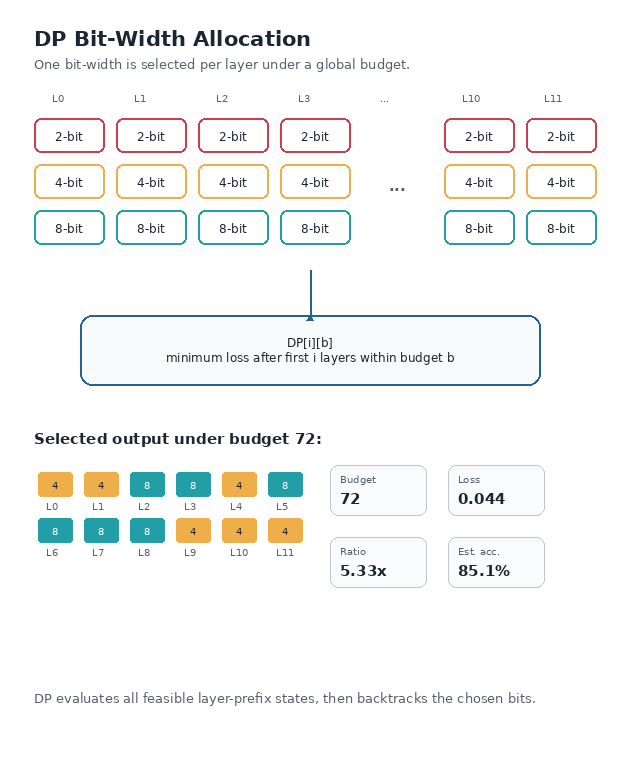
\includegraphics[width=\columnwidth]{figures/dp_allocation_diagram_column.png}}
\caption{Dynamic Programming view of mixed-precision allocation. Each layer contributes one group of bit-width choices, and the DP table selects the minimum-loss configuration under the global budget.}
\label{fig:dpallocation}
\end{figure}

\section{Methodology}
\subsection{Experimental Pipeline}
The experiment is designed to connect an actual Transformer model with an algorithmic allocation procedure. BERT-base is used as the target model because it has twelve Transformer encoder layers, making the layer-wise allocation problem large enough to demonstrate the value of Dynamic Programming. The model is fine-tuned on the SST-2 sentiment classification task from the GLUE benchmark using a subset of 2000 training samples and evaluated on 500 validation samples. The objective of the experiment is not to maximize SST-2 accuracy, but to obtain a realistic sensitivity profile for the Transformer layers under different fake-quantized bit-widths.

The experimental pipeline consists of five stages. First, BERT-base is loaded with a sequence classification head and evaluated to obtain baseline accuracy and F1-score. Second, the model is fine-tuned for one epoch to adapt it to the SST-2 binary classification task. Third, each Transformer layer is fake-quantized independently using bit-widths $\{2,4,8\}$ while the remaining layers stay at their current precision. Fourth, each fake-quantized model variant is evaluated to estimate the accuracy loss caused by that layer-bit pair. Finally, the resulting sensitivity table is passed to Dynamic Programming, greedy, and uniform baselines.

\subsection{Layer-Wise Sensitivity Measurement}
For each Transformer layer $i$ and bit-width $q$, the experiment temporarily replaces the weights of layer $i$ with fake-quantized weights. After evaluation, the original weights are restored before testing the next configuration. This ensures that each sensitivity measurement isolates one layer-bit pair rather than accumulating quantization effects across multiple layers.

The validation accuracy loss is computed as
\begin{equation}
d_i(q)=\max(0,A_{\mathrm{base}}-A_i(q)),
\end{equation}
where $A_{\mathrm{base}}$ is the baseline validation accuracy and $A_i(q)$ is the validation accuracy after layer $i$ is fake-quantized to $q$ bits. The maximum operation prevents small evaluation noise from producing negative loss values. Each BERT-base Transformer layer contains 7,087,872 trainable parameters in the evaluated configuration, so the relative size of one layer under bit-width $q$ is represented by $q$.

\subsection{Dynamic Programming Allocator}
The Dynamic Programming allocator receives the sensitivity table as input. Each layer must choose exactly one bit-width from $Q=\{2,4,8\}$. Since all optimized layers have equal parameter count in BERT-base, the relative cost of choosing bit-width $q$ is simply $q$. A budget $B$ therefore represents the maximum sum of selected bit-widths across the twelve optimized layers.

Algorithmically, the allocator initializes $DP[0][b]=0$ for all budget values $b$. For each layer $i$, each budget $b$, and each candidate bit-width $q$, it updates the DP table using the recurrence defined in the theoretical foundation. A parent table stores the selected bit-width so that the final configuration can be reconstructed by backtracking from $DP[L][B]$. In the experiment, budgets $\{48,56,60,64,72\}$ are evaluated to observe how the selected configuration changes as the compression constraint is relaxed.

\subsection{Baseline Methods}
Three baselines are used. Uniform 2-bit, 4-bit, and 8-bit quantization assign the same bit-width to every optimized layer. These baselines measure the effect of simple non-adaptive compression. The greedy baseline starts from the all-8-bit configuration and repeatedly lowers the bit-width of the layer that gives the smallest additional accuracy loss per unit of size saved. This represents a locally optimal heuristic. The proposed DP method differs from greedy because it evaluates the global optimum under each budget, rather than committing to a sequence of local compression choices.

\subsection{Evaluation Metrics}
The experiment reports five metrics: selected bit configuration, total relative size, compression ratio against 32-bit storage, estimated accuracy loss, and estimated post-allocation accuracy. The compression ratio is computed as
\begin{equation}
R=\frac{32L}{\sum_{i=1}^{L}q_i},
\end{equation}
where $L=12$ for BERT-base Transformer layers. Estimated post-allocation accuracy is computed as
\begin{equation}
A_{\mathrm{est}}=A_{\mathrm{base}}-\sum_{i=1}^{L}d_i(q_i).
\end{equation}
This estimate relies on the additive loss assumption, which is useful for DP formulation but may not perfectly match the accuracy of jointly quantizing all selected layers. The paper therefore interprets the result as a budget-aware sensitivity estimate rather than a hardware deployment benchmark.

\section{Results and Discussion}
\subsection{Baseline Accuracy}
After fine-tuning on the SST-2 subset, BERT-base achieves approximately 89.4\% validation accuracy. This baseline represents the reference model before mixed-precision allocation. Since the experiment focuses on compression rather than state-of-the-art SST-2 performance, the baseline is sufficient for observing how different layers respond to fake quantization.

\subsection{Layer Sensitivity}
Figure \ref{fig:sensitivity} visualizes the measured accuracy loss after fake quantizing each individual BERT-base layer. The result shows that 8-bit fake quantization is almost lossless, while 2-bit quantization is destructive for most layers. Several 2-bit configurations produce losses above 0.40, meaning that the model nearly collapses to random-like behavior on the validation subset. In contrast, many 4-bit configurations remain close to the full-precision baseline, with losses between 0.000 and 0.034. This confirms the main motivation for mixed precision: different Transformer layers tolerate low precision differently, and the allocation should not be uniform.

\begin{figure*}[htbp]
\centerline{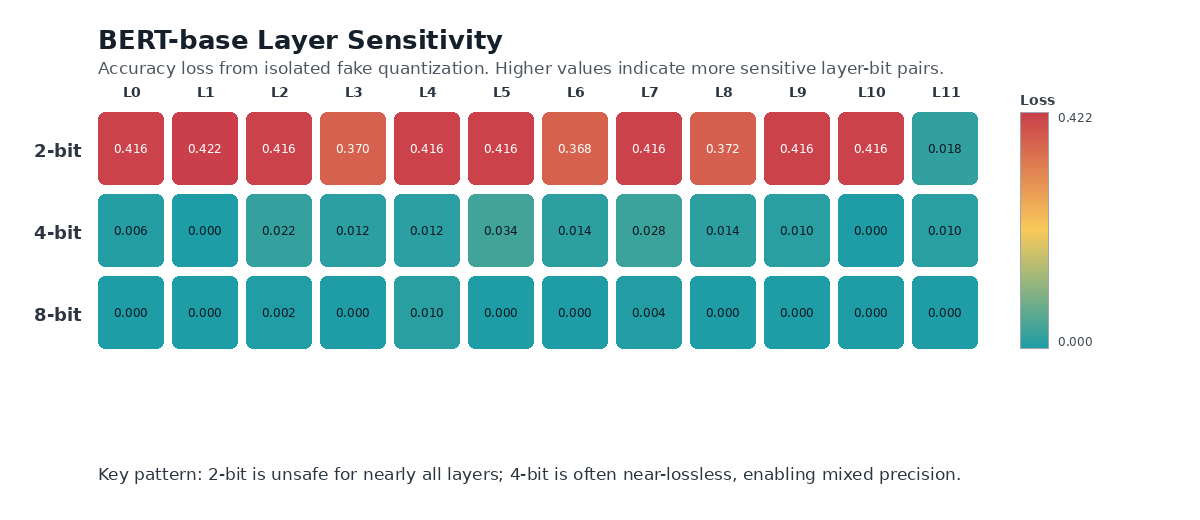
\includegraphics[width=0.92\textwidth]{figures/bertbase_sensitivity_heatmap.png}}
\caption{Layer-wise BERT-base accuracy loss under fake quantization. Redder cells indicate more sensitive layer-bit pairs.}
\label{fig:sensitivity}
\end{figure*}

The sensitivity pattern is especially important for the optimization problem. If uniform 2-bit quantization is applied, every layer is compressed aggressively, including highly sensitive layers. This leads to an estimated aggregate loss of 4.462, making it unsuitable despite its 16.00$\times$ theoretical compression ratio. However, the DP allocator can avoid 2-bit assignments and selectively preserve 8-bit precision on the layers where the marginal loss reduction is worth the additional budget. The experiment therefore provides evidence that bit-width allocation should be treated as a global optimization problem rather than a uniform rule.

\subsection{Allocation Results}
Table \ref{tab:allocation} reports the selected DP configuration for each budget. The best trade-off used as the main result is budget 72, where DP selects $[4,4,8,8,4,8,8,8,8,4,4,4]$. This configuration keeps layers 2, 3, 5, 6, 7, and 8 at 8-bit precision while compressing the remaining layers to 4-bit. The total relative size is 72, corresponding to a 5.33$\times$ compression ratio compared with 32-bit storage. The estimated accuracy loss is 0.044, giving an estimated accuracy of 85.1\%.

\begin{table}[htbp]
\caption{DP Allocation Under Different Budgets}
\begin{center}
\begin{tabular}{|c|c|c|c|c|}
\hline
\textbf{Budget} & \textbf{Config} & \textbf{Ratio} & \textbf{Loss} & \textbf{Est. Acc.} \\
\hline
48 & [4,4,4,4,4,4,4,4,4,4,4,4] & 8.00$\times$ & 0.162 & 73.3\% \\
56 & [4,4,4,4,4,8,4,8,4,4,4,4] & 6.86$\times$ & 0.104 & 79.1\% \\
60 & [4,4,8,4,4,8,4,8,4,4,4,4] & 6.40$\times$ & 0.084 & 81.1\% \\
64 & [4,4,8,4,4,8,8,8,4,4,4,4] & 6.00$\times$ & 0.070 & 82.5\% \\
72 & [4,4,8,8,4,8,8,8,8,4,4,4] & 5.33$\times$ & 0.044 & 85.1\% \\
\hline
\end{tabular}
\label{tab:allocation}
\end{center}
\end{table}

Figure \ref{fig:tradeoff} shows the compression-accuracy trade-off across evaluated budgets. The budget-72 result is the most balanced configuration. It provides substantial compression while avoiding the severe degradation caused by 2-bit quantization in sensitive layers. Compared with the 32-bit baseline, the estimated storage requirement is reduced by more than five times. Compared with uniform 4-bit quantization, which achieves 8.00$\times$ compression but only 73.3\% estimated accuracy, the budget-72 DP configuration sacrifices some compression to preserve far more predictive performance.

\begin{figure*}[htbp]
\centerline{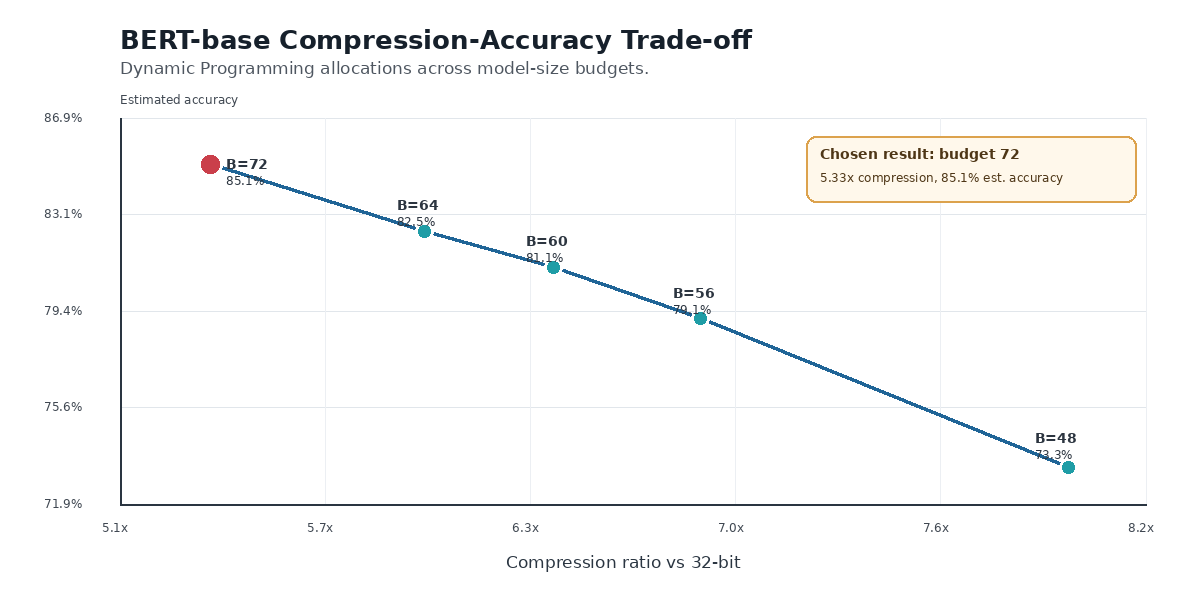
\includegraphics[width=0.92\textwidth]{figures/bertbase_tradeoff.png}}
\caption{Dynamic Programming trade-off curve for BERT-base. Higher compression produces lower estimated accuracy, while the selected budget-72 configuration preserves 85.1\% estimated accuracy at 5.33$\times$ compression.}
\label{fig:tradeoff}
\end{figure*}

\subsection{Comparison with Greedy and Uniform Baselines}
At tight budgets, DP provides better allocation than greedy. For budget 48, DP selects the all-4-bit configuration with estimated loss 0.162, while greedy selects a configuration ending in one 2-bit layer with loss 0.170. For budget 56, DP selects $[4,4,4,4,4,8,4,8,4,4,4,4]$ with loss 0.104, while greedy selects $[4,4,4,4,4,8,4,8,4,4,4,2]$ with loss 0.112. These results show that greedy can over-compress a layer because it follows local loss-per-size decisions, while DP evaluates the complete configuration under the budget.

For budgets 60, 64, and 72, greedy happens to match the DP loss, although at budget 64 it reaches the same loss with a slightly different configuration. This does not weaken the DP formulation; rather, it shows that the greedy heuristic can sometimes find an equally good solution on this sensitivity landscape. The advantage of DP is its optimality guarantee. Once the sensitivity table and budget are fixed, DP returns the minimum-loss feasible configuration under the additive assumption. Greedy cannot provide this guarantee, and the budget-48 and budget-56 cases show concrete instances where it is suboptimal.

\subsection{Interpretation}
The selected budget-72 configuration reveals a meaningful compression pattern. No layer is assigned 2-bit because the measured 2-bit losses are too large for BERT-base on this task. The allocator instead chooses between 4-bit and 8-bit precision. Layers 2, 3, 5, 6, 7, and 8 receive 8-bit because their 4-bit alternatives introduce larger losses relative to the available budget. Layers 0, 1, 4, 9, 10, and 11 are compressed to 4-bit because their measured 4-bit losses are small enough to justify the storage saving. This behavior matches the intended role of mixed-precision quantization: preserve precision where it matters and compress where the model can tolerate it.

The experiment also demonstrates the practical limitation of the additive sensitivity assumption. The reported estimated accuracy is computed by summing individual layer losses. In a real jointly quantized model, interactions between quantized layers may increase or decrease the final accuracy loss. Nevertheless, the additive table is valuable for algorithmic allocation because it transforms layer sensitivity into a structured optimization problem solvable by Dynamic Programming.

\section{Conclusion}
This paper formulates mixed-precision bit-width allocation for Transformer compression as a multiple-choice knapsack-style optimization problem. Each BERT-base Transformer layer is assigned one bit-width from $\{2,4,8\}$, with storage cost as the constraint and fake-quantization accuracy loss as the optimization objective. Dynamic Programming is used to recover the minimum-loss feasible configuration under each model-size budget.

Experiments on BERT-base with SST-2 validation data show that Transformer layers have different quantization sensitivities. Most layers suffer severe degradation at 2-bit precision, while many layers remain usable at 4-bit. Under the selected budget 72, the proposed DP allocator chooses $[4,4,8,8,4,8,8,8,8,4,4,4]$, achieving an estimated 5.33$\times$ compression ratio with 0.044 accuracy loss from an 89.4\% baseline. This corresponds to an estimated post-allocation accuracy of 85.1\%.

The results show that DP is most useful when budget constraints make local decisions unreliable. At budgets 48 and 56, DP outperforms the greedy baseline by finding lower-loss configurations. At larger budgets, greedy matches DP or reaches the same loss on this instance, but DP retains the stronger guarantee of global optimality under the additive loss model.

The main limitation is that fake quantization evaluates the effect of reduced precision without implementing hardware-level low-bit inference. Therefore, the reported compression ratios estimate weight storage reduction, not actual end-to-end latency improvement. Another limitation is the additive loss assumption: the final behavior of jointly quantized layers may differ from the sum of individual layer sensitivities. Future work can evaluate the selected DP configurations with actual joint quantization, include activation quantization, and test larger Transformer families or encoder-decoder architectures.

\section*{Appendix}
\subsection*{A. Experiment Artifacts}
The main experiment notebook is provided in the \texttt{notebooks/} directory as \texttt{bitweaver\_bert\_base\_experiment.ipynb}. The generated sensitivity and comparison CSV files are stored under \texttt{docs/bert-base/}. The complete project repository is available at \url{https://github.com/AthillaZaidan/TransformerCompression}.

\section*{Acknowledgment}
The author thanks the lecturers and assistants of IF2211 Strategi Algoritma for providing the academic framework that made this project possible. The author also thanks family and friends for their support throughout the writing and experimentation process.

\begin{thebibliography}{00}
\bibitem{transformer} A. Vaswani, N. Shazeer, N. Parmar, J. Uszkoreit, L. Jones, A. N. Gomez, L. Kaiser, and I. Polosukhin, ``Attention is all you need,'' in \textit{Advances in Neural Information Processing Systems}, vol. 30, 2017.
\bibitem{bert} J. Devlin, M.-W. Chang, K. Lee, and K. Toutanova, ``BERT: Pre-training of deep bidirectional transformers for language understanding,'' in \textit{Proc. North American Chapter of the Association for Computational Linguistics}, 2019, pp. 4171--4186.
\bibitem{haq} K. Wang, Z. Liu, Y. Lin, J. Lin, and S. Han, ``HAQ: Hardware-aware automated quantization with mixed precision,'' in \textit{Proc. IEEE/CVF Conference on Computer Vision and Pattern Recognition}, 2019, pp. 8612--8620.
\bibitem{qbert} S. Shen, Z. Dong, J. Ye, L. Ma, Z. Yao, A. Gholami, M. W. Mahoney, and K. Keutzer, ``Q-BERT: Hessian based ultra low precision quantization of BERT,'' in \textit{Proc. AAAI Conference on Artificial Intelligence}, vol. 34, no. 5, 2020, pp. 8815--8821.
\bibitem{zeroquant} Z. Yao, R. Y. Aminabadi, M. Zhang, X. Wu, C. Li, and Y. He, ``ZeroQuant: Efficient and affordable post-training quantization for large-scale transformers,'' in \textit{Advances in Neural Information Processing Systems}, vol. 35, 2022, pp. 27168--27183.
\bibitem{martello} S. Martello and P. Toth, \textit{Knapsack Problems: Algorithms and Computer Implementations}. Chichester, U.K.: Wiley, 1990.
\end{thebibliography}

\section*{Statement}
I hereby declare that this paper is an original work, written on my own, and does not involve plagiarism, unauthorized adaptation, or translation of another individual's work.

\vspace{10pt}
\begin{samepage}
\noindent Bandung, 19 June 2026

\vspace{4pt}
\noindent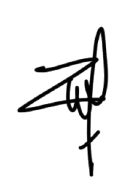
\includegraphics[width=0.26\columnwidth]{figures/tanda-tangan.png}

\vspace{2pt}
\noindent Athilla Zaidan Zidna Fann, 13524068
\end{samepage}

\end{document}
